\documentclass[11pt,a4paper]{article}

\usepackage[margin=25mm]{geometry}
\usepackage[T1]{fontenc}
\usepackage[utf8]{inputenc}
\usepackage{lmodern}
\usepackage{microtype}
\usepackage{amsmath,amssymb}
\usepackage{booktabs,longtable,tabularx,array}
\usepackage{graphicx}
\usepackage{tikz}
\usetikzlibrary{arrows.meta,positioning,fit}
\usepackage{xcolor}
\usepackage{enumitem}
\usepackage{xurl}
\usepackage{hyperref}
\usepackage{fancyhdr}
\usepackage{caption}
\usepackage{listings}

\definecolor{skysealgreen}{HTML}{173F33}
\definecolor{skysealgray}{HTML}{5D6964}
\definecolor{skyseallight}{HTML}{EDF3F0}
\definecolor{codegray}{HTML}{F4F5F5}

\hypersetup{
  colorlinks=true,
  linkcolor=skysealgreen,
  citecolor=skysealgreen,
  urlcolor=skysealgreen,
  pdftitle={SkySeal: Identity-Bound Timestamping of Private Research Files with a Himawari Earth-State Witness},
  pdfauthor={Katsushi Kagaya},
  pdfsubject={SkySeal technical report, version 1.0},
  pdfkeywords={digital timestamping, research provenance, WebAuthn, passkey, ORCID, OpenTimestamps, Himawari}
}

\pagestyle{fancy}
\fancyhf{}
\fancyhead[L]{\small SkySeal Technical Report v1.0}
\fancyhead[R]{\small 30 August 2026}
\fancyfoot[C]{\thepage}
\setlength{\headheight}{14pt}
\setlength{\parindent}{0pt}
\setlength{\parskip}{0.55em}
\setlist[itemize]{leftmargin=1.6em,itemsep=1pt,topsep=4pt}
\setlist[enumerate]{leftmargin=1.6em,itemsep=1pt,topsep=4pt}
\captionsetup{font=small,labelfont=bf}

\newcommand{\code}[1]{\texttt{\detokenize{#1}}}
\newcommand{\sha}{\operatorname{SHA256}}
\newcommand{\jcs}{\operatorname{JCS}}
\newcommand{\claim}{\textbf{Verifiable claim.}}
\newcommand{\nonclaim}{\textbf{Non-claim.}}

\lstset{
  basicstyle=\ttfamily\footnotesize,
  backgroundcolor=\color{codegray},
  frame=single,
  rulecolor=\color{skyseallight},
  breaklines=true,
  columns=fullflexible,
  keepspaces=true,
  showstringspaces=false,
  xleftmargin=0.4em,
  xrightmargin=0.4em,
  aboveskip=0.8em,
  belowskip=0.8em
}

\begin{document}
\pagenumbering{gobble}

\begin{titlepage}
\centering
\vspace*{18mm}
{\color{skysealgreen}\rule{0.86\textwidth}{1.2pt}}\\[13mm]
{\Huge\bfseries SkySeal\\[3mm]}
{\LARGE Identity-Bound Timestamping of Private Research Files\\[2mm]
with a Himawari Earth-State Witness\par}
\vspace{12mm}
{\Large Technical Report, Version 1.0\par}
\vspace{4mm}
{\large 30 August 2026\par}
\vfill
{\Large Katsushi Kagaya\par}
\vspace{2mm}
{\normalsize Kitami Institute of Technology, Japan\par}
{\normalsize \href{mailto:kkagaya@mail.kitami-it.ac.jp}{kkagaya@mail.kitami-it.ac.jp}\par}
{\normalsize ORCID: \href{https://orcid.org/0000-0003-3001-7690}{0000-0003-3001-7690}\par}
\vspace{12mm}
{\normalsize Reference implementation:\par}
{\normalsize \url{https://github.com/kagaya/SkySeal}\par}
\vfill
{\color{skysealgreen}\rule{0.86\textwidth}{1.2pt}}\\[5mm]
{\small Implementation baseline: SkySeal protocol v1.2.0-draft.1, commit \code{d0b2953f0929}.}
\end{titlepage}
\pagenumbering{roman}

\begin{abstract}
Digital research objects are easy to copy, revise, and synthesize, while conventional file metadata is easy to alter and often disappears when a file is moved. SkySeal is a deployable timestamping and research-provenance system that creates public, independently verifiable evidence about private files without publishing their contents, names, paths, or Google Drive identifiers. A private agent streams file bytes from a dedicated Google Drive inbox, commits to a sorted set of SHA-256 digests, and requests explicit approval. The approval is a User-Present and User-Verified WebAuthn assertion made with a Passkey whose public key is activated together with an authenticated ORCID iD. The resulting evidence bundle is timestamped with OpenTimestamps, persisted first on an HTTPS server, and mirrored to a public GitHub repository. An optional owner-only ledger preserves the private correspondence between a Drive object and its public seal.

SkySeal v1.2 adds the element from which the system takes its name: a recent Japan Meteorological Agency Himawari-8/9 full-disk Band 13 infrared image. The exact image digest and observation metadata are included in the Passkey-signed payload. This sky witness supplies human-inspectable physical context and, conditional on JMA provenance and the capture controls, a lower temporal bound. A confirmed Bitcoin-backed OpenTimestamps proof supplies an independent upper bound. The sky image is not itself a trustless timestamp and does not replace OpenTimestamps.

This report specifies the claim semantics, protocol, trust boundaries, public evidence format, verification procedure, privacy properties, and limitations of SkySeal. It also documents the first production v1.2 seal. The central claim is deliberately narrow: exact disclosed bytes can be shown to belong to a hash set that was explicitly approved by the Passkey associated with a particular authenticated ORCID identity, and, after timestamp confirmation, that signed evidence existed before an independently attested blockchain time. SkySeal does not by itself prove authorship, ownership, scientific correctness, exclusive possession, or the exact time at which a work was created.
\end{abstract}

\tableofcontents
\clearpage
\pagenumbering{arabic}

\section{Introduction}

The classical digital timestamping problem is to establish temporal evidence about data rather than about a storage medium. Haber and Stornetta formulated this problem for documents stored on easily modifiable media and proposed cryptographic linking and public commitment mechanisms \cite{haber1991}. A trusted time-stamping authority can similarly attest that a digest existed before a stated time, as standardized in RFC 3161 \cite{rfc3161}. OpenTimestamps instead aggregates commitments and anchors them in Bitcoin, allowing later independent verification against a public proof-of-work history \cite{nakamoto2008,ots2026}.

Research provenance adds a second problem: a timestamp should be connected to a researcher in a way that remains usable after devices, institutions, and software environments change. A conventional account login is insufficient as a durable public proof, while publishing source files merely to obtain a date can violate confidentiality or premature-disclosure constraints. SkySeal addresses this gap by combining four evidence layers:

\begin{enumerate}
  \item a byte-level SHA-256 commitment to a private file or file set;
  \item an identity activation that combines an authenticated ORCID iD with a User-Verified Passkey;
  \item an explicit WebAuthn approval over the exact canonical seal payload;
  \item independently verifiable public evidence, including OpenTimestamps and a contemporaneous Himawari Earth-state witness.
\end{enumerate}

The design is motivated by research priority, laboratory records, preprints, analysis outputs, and other objects for which exact bytes may need to be authenticated later. The rapid growth of synthetic media makes such evidence more valuable, but also makes overstatement dangerous. SkySeal therefore separates a cryptographically checkable statement from interpretations such as ``the named researcher authored this work.''

The implementation described here is operational at \url{https://proof.excyberlab.net}. It uses a private Google Drive inbox, an always-on Linux virtual private server (VPS), ORCID OAuth, an iPhone Passkey, a Python reference service and verifier, OpenTimestamps, a VPS public evidence store, and a GitHub mirror \cite{skyseal2026}.

\section{Design objectives and explicit non-objectives}

\subsection{Objectives}

SkySeal is designed to satisfy the following practical requirements.

\begin{itemize}
  \item \textbf{Private-source operation.} Original bytes, file names, paths, directory topology, Drive IDs, and file-to-hash mappings are not published.
  \item \textbf{Byte-exact auditability.} A later auditor can hash a disclosed candidate and test whether its exact bytes were committed.
  \item \textbf{Explicit human approval.} An unattended agent may prepare a transaction, but publication requires a User-Present and User-Verified WebAuthn assertion.
  \item \textbf{Researcher identifier binding.} The public credential history is bound to an ORCID iD obtained through OAuth rather than manual text entry \cite{orcid2026}.
  \item \textbf{Independent survival.} The public evidence is useful without the private Drive folder, owner-only ledger, original VPS database, or access to the Passkey.
  \item \textbf{Redundant publication.} Complete packages are persisted on the VPS before best-effort mirroring to GitHub.
  \item \textbf{Physical context.} A recent full-disk infrared view of Earth is included in the signed payload and public package.
\end{itemize}

\subsection{Non-objectives}

SkySeal is not a qualified electronic-signature service, a certificate authority, a notarization service, or a substitute for scientific review. It does not establish:

\begin{itemize}
  \item who intellectually authored or owns the committed content;
  \item whether the content is correct, original, ethical, or complete;
  \item the exact wall-clock time at which the content was first created;
  \item exclusive possession or the absence of earlier copies;
  \item file names, paths, ordering, hierarchy, or multiplicity from the public hash set;
  \item an immutable storage guarantee for the original file.
\end{itemize}

These exclusions are part of the protocol interpretation, not incidental disclaimers.

\section{Relationship to existing provenance mechanisms}

SkySeal occupies a specific point among timestamping and provenance systems. RFC 3161 defines a request and signed response involving a Time-Stamping Authority, with the authority acting as a trusted third party \cite{rfc3161}. OpenTimestamps creates a different trust model: remote calendars aggregate commitments, while the final proof is verified using a Bitcoin block attestation rather than the calendar's wall clock \cite{ots2026,otsclient2026}. SkySeal uses this latter model for the upper time bound.

Content Credentials based on C2PA bind provenance assertions to media assets and support a broader ecosystem of signed claims and editing history \cite{c2pa2026}. SkySeal is complementary. It is optimized for a private source file or private set whose public representation is a minimal hash commitment. It does not embed a provenance manifest in the source asset, and it intentionally withholds descriptive metadata.

WebAuthn standardizes public-key credentials scoped to a relying party and supports registration and assertion ceremonies \cite{w3c2026}. Passkeys make this mechanism accessible through platform authenticators and cross-device flows \cite{fido2026}. SkySeal uses WebAuthn not merely to log into a service but to approve a domain-separated digest of a canonical protocol payload. ORCID supplies a persistent researcher identifier, while the Passkey supplies proof that the activated credential approved a specific seal. Neither layer alone is treated as the full identity statement.

The Himawari witness is intentionally distinct from these cryptographic systems. JMA performs full-disk observations every ten minutes \cite{jma2026}. SkySeal records one recent Band 13 infrared image, available day and night, and binds its exact bytes to the approval. The image makes the evidence physically interpretable and places the digital event beside a state of Earth. However, because JMA does not provide a SkySeal-specific cryptographic signature and a historical image could be attached later, this component is conditional evidence rather than a replacement for blockchain anchoring.

\section{System architecture}

Figure~\ref{fig:architecture} shows the production data flow. The private Drive agent is the only component that reads source bytes. The public service receives the digest of the strict hash-list bytes, the number of distinct hashes, protocol state, the optional private-ledger commitment, and the sky-witness metadata. JMA receives only an ordinary HTTPS request for a public image and receives no file hash, Drive identifier, or ORCID value.

\begin{figure}[htbp]
\centering
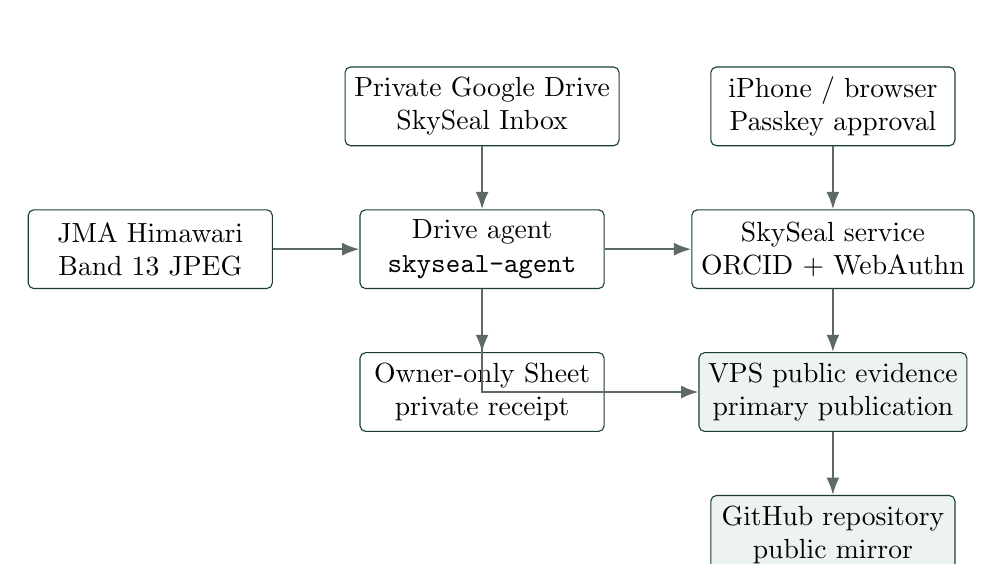
\begin{tikzpicture}[
  node distance=8mm and 11mm,
  box/.style={draw=skysealgreen, rounded corners=2pt, align=center, minimum height=10mm, minimum width=31mm, fill=white},
  pub/.style={box, fill=skyseallight},
  arrow/.style={-{Latex[length=2.2mm]}, thick, draw=skysealgray},
  label/.style={font=\scriptsize, text=skysealgray, align=center}
]
\node[box] (drive) {Private Google Drive\\SkySeal Inbox};
\node[box, below=of drive] (agent) {Drive agent\\\code{skyseal-agent}};
\node[box, left=of agent] (jma) {JMA Himawari\\Band 13 JPEG};
\node[box, right=of agent] (service) {SkySeal service\\ORCID + WebAuthn};
\node[box, above=of service] (phone) {iPhone / browser\\Passkey approval};
\node[box, below=of agent] (ledger) {Owner-only Sheet\\private receipt};
\node[pub, below=of service] (vps) {VPS public evidence\\primary publication};
\node[pub, below=of vps] (github) {GitHub repository\\public mirror};

\draw[arrow] (drive) -- (agent);
\draw[arrow] (jma) -- (agent);
\draw[arrow] (agent) -- (service);
\draw[arrow] (phone) -- (service);
\draw[arrow] (service) -- (vps);
\draw[arrow] (agent) -- (ledger);
\draw[arrow] (agent) |- (vps);
\draw[arrow] (vps) -- (github);
\end{tikzpicture}
\caption{SkySeal production architecture. Green-tinted nodes are public evidence stores; source content remains within the private Drive/agent boundary.}
\label{fig:architecture}
\end{figure}

\subsection{Principal components}

\begin{longtable}{>{\raggedright\arraybackslash}p{0.21\textwidth}>{\raggedright\arraybackslash}p{0.35\textwidth}>{\raggedright\arraybackslash}p{0.35\textwidth}}
\toprule
Component & Function & Sensitive state \\
\midrule
\endhead
Google Drive inbox & Holds source objects and defines sealing units by direct children. & Original bytes, names, hierarchy, IDs, revisions. \\
Drive agent & Waits for stability, streams and hashes bytes, captures the sky witness, polls approval, verifies, timestamps, and publishes. & Drive token, service-account key, transaction bearer, private snapshot and hash mapping. \\
SkySeal service & Runs ORCID OAuth, WebAuthn registration and assertions, transaction state, and public identity records. & Session data, raw credential routing IDs, agent-token hash. \\
Passkey authenticator & Protects the private credential and produces User-Present/User-Verified assertions. & Private credential key. \\
JMA endpoint & Supplies the recent public Himawari image. & No SkySeal secrets are sent. \\
VPS evidence store & Serves complete public packages before GitHub mirroring. & Public artifacts only. \\
GitHub mirror & Provides an additional public copy and repository history. & Public artifacts only. \\
Private ledger & Optionally maps a private Drive root object to a public seal through a salted receipt. & Root name, Drive ID/link, receipt salt and JSON. \\
\bottomrule
\end{longtable}

The web service and Drive agent run under separate Linux users. The agent services set \code{MemorySwapMax=0} and \code{LimitCORE=0}, preventing service swap and core dumps. This reduces accidental persistence of streamed source bytes but does not protect against a compromised root account, operating system, hypervisor, or storage administrator.

\section{Protocol}

\subsection{Identity enrollment and activation}

Enrollment begins with ORCID OAuth using the \code{/authenticate} scope. The returned authenticated ORCID iD is validated and stored; access and refresh tokens are discarded by the reference implementation. The user then registers a WebAuthn credential. Registration requires user verification and uses no attestation statement (\code{attestation = none}), so the public proof does not claim a particular authenticator make or hardware provenance.

Registration creates a public identity-genesis object containing the authenticated ORCID iD, relying-party identifier, public credential key, recovery-code commitment, version, and timestamps. The raw credential ID and stable user handle remain private. A second User-Verified assertion activates this exact genesis. If $G$ is the canonical identity-genesis object and $A$ is the activation payload, the activation challenge is

\begin{equation}
c_A = \sha\!\left(
  \operatorname{UTF8}(\texttt{"SkySeal Identity Activation Challenge v1"})
  \parallel \mathtt{0x00} \parallel \jcs(A)
\right),
\end{equation}

where $\parallel$ denotes byte concatenation and JCS is RFC 8785 canonical JSON \cite{rfc8785}. The activation payload includes $\sha(\jcs(G))$, thereby binding the assertion to the published public key and ORCID identity. Production identity is therefore expressed as:

\begin{equation}
\text{authenticated ORCID account}
\quad + \quad
\text{User-Verified control of the activated Passkey}.
\end{equation}

The current production identity is \url{https://orcid.org/0000-0003-3001-7690}. An OpenPGP fingerprint may remain as legacy metadata in an existing genesis, but OpenPGP proof of control is not required for v1.2.

\subsection{Drive stability and byte hashing}

Each direct child of the inbox is one sealing unit. A direct file is a one-member unit; a direct folder is recursively traversed and all non-folder descendants form one unit. Empty folders are not submitted, and shortcuts are rejected. The agent computes a private snapshot from identifiers, MIME types, revision state, sizes, checksums, modification state, and parent relationships. It requires the snapshot to remain unchanged for 120 seconds.

Ordinary binary files are downloaded as a stream and read in 1 MiB chunks. The agent does not intentionally write the complete source to disk and does not load a large ordinary file into memory at once. If Drive supplies \code{sha256Checksum}, the independently calculated digest must match it. Google Workspace objects are exported to fixed representations: Docs to PDF, Sheets to XLSX, Slides to PDF, and Drawings to PDF. The commitment is to those exact export bytes, not to an abstract editor document. Google documents exceeding the ordinary export limit must first be stored as ordinary files \cite{gdrive2026}.

For member byte strings $F_1,\ldots,F_n$, the agent computes

\begin{equation}
h_i = \sha(F_i).
\end{equation}

It removes duplicate digests, sorts the remaining lowercase hexadecimal values lexicographically, and writes one 64-character digest plus LF per line. Let those exact bytes be $L$. The public subject commitment is

\begin{equation}
d_S = \sha(L).
\end{equation}

This construction commits to a mathematical set of distinct content digests. It deliberately discards order, path, directory topology, and multiplicity. After hashing, the agent re-inventories the Drive unit; any intervening change invalidates the attempt.

\subsection{Himawari sky witness}

The production configuration requires a sky witness. The agent rounds a time initially 20 minutes before retrieval down to a ten-minute UTC slot, then tries up to ten progressively earlier slots. For each candidate it retrieves the JMA full-disk Band 13 infrared JPEG. Band 13 is used because infrared imagery remains useful both day and night.

The JMA URL contains only \code{HHMM} and is reused daily. The agent therefore rejects a response unless:

\begin{itemize}
  \item \code{Last-Modified} is parseable and falls between the intended observation time and six hours after it;
  \item the HTTP media type is \code{image/jpeg};
  \item the byte stream has complete JPEG start and end markers;
  \item the size is between 1 KiB and 2 MiB.
\end{itemize}

The resulting strict metadata object $W$ records the provider, platform series, product, observation time, retrieval time, source URL, media type, attribution, and

\begin{equation}
d_I = \sha(\text{exact JPEG bytes}).
\end{equation}

Both $W$ and the JPEG are retained by the private agent until publication. If no candidate passes, seal creation fails closed and the system retries during a later timer run. All ready units processed in one scan reuse the same captured observation, which limits unnecessary requests and gives those units a common physical context.

\subsection{Seal approval}

The seal payload $P$ contains the UUIDv7 seal identifier, commitment format, $d_S$, ORCID identity, identity version, activation-state digest, a 256-bit nonce, an informational server time, the optional private-ledger commitment, and the complete sky-witness object $W$. The approval challenge is

\begin{equation}
c_S = \sha\!\left(
  \operatorname{UTF8}(\texttt{"SkySeal WebAuthn Challenge v1"})
  \parallel \mathtt{0x00} \parallel \jcs(P)
\right).
\end{equation}

The browser requests a WebAuthn assertion. The service verifies the exact HTTPS origin, RP-ID hash, challenge, non-cross-origin status, User Present flag, User Verified flag, credential ownership, and the ES256 or Ed25519 signature. The public bundle omits the raw credential ID and user handle. The current production credential uses ES256 with a P-256 public key.

The browser displays the Seal ID, distinct-hash count, state, expiry, and Himawari observation time. It does not receive the source name, path, or bytes. This privacy decision means that user approval confirms the presented transaction and count but does not itself visually prove which private Drive object the agent hashed; faithful ingestion remains within the trusted computing base.

\subsection{Timestamping and publication}

After approval, the agent retrieves the hash list, seal bundle, identity genesis, and identity activation. Before publication it independently checks the hash commitment, identity digests, WebAuthn signature, expected RP ID, exact origin, and activation proof.

OpenTimestamps stamps the exact bytes of \nolinkurl{seal.skyseal.json} and \nolinkurl{identity-activation.json}. Initial receipts may contain pending calendar attestations. A daily upgrade process later incorporates Bitcoin confirmation; only the \code{.ots} files and manifest may change during this upgrade. A valid confirmation establishes that the target bytes existed before the attested Bitcoin block time \cite{ots2026}. It does not establish the exact creation time.

The package is written atomically to the VPS public root and then mirrored to GitHub, with the manifest sent last. A GitHub failure does not undo local publication. The private state records a pending mirror and retries later. Existing evidence cannot be overwritten with different bytes; publication is idempotent.

\subsection{Optional owner-only ledger}

Public minimalism makes file-name correspondence private by design. When the owner-only ledger is enabled, the agent constructs a receipt $R$ containing the direct-child Drive ID, display name and link, root MIME type, private snapshot digest, public subject digest, entry count, and a random 256-bit salt. The public seal contains only

\begin{equation}
d_R = \sha(\jcs(R)).
\end{equation}

Because the random salt is part of $R$, predictable names and Drive IDs cannot be tested directly against $d_R$. The full receipt is appended idempotently to a non-public Google Sheet after local publication. Selective disclosure of a receipt later proves the private/public correspondence. The ledger is not required for byte-membership verification and is not an end-to-end encrypted vault; the owner, explicitly shared service account, and sufficiently privileged VPS or organizational administrators can technically read it.

\section{Public evidence and independent verification}

\subsection{Publication package}

A v1.2 package contains nine files:

\begin{lstlisting}
evidence/YYYY/MM/<seal-id>/
  hashes.txt
  seal.skyseal.json
  seal.skyseal.json.ots
  identity-genesis.json
  identity-activation.json
  identity-activation.json.ots
  sky-witness.json
  sky-witness.jpg
  manifest.json
\end{lstlisting}

The manifest records the SHA-256 digest of every other artifact and the two proof-to-target relationships. The standalone verifier reads no private server database and makes no Google Drive request. The auditor supplies the expected RP ID and origin from a trusted local choice; values inside the bundle are treated only as hints.

\subsection{Claim semantics}

For a disclosed candidate $F$, successful complete verification establishes the following chain:

\begin{enumerate}
  \item $\sha(F)$ appears in the strict hash set $L$;
  \item $\sha(L)$ equals the subject digest in the canonical seal payload;
  \item the payload includes the identity-state digest and exact sky-witness metadata;
  \item the WebAuthn assertion is valid for the expected origin and RP ID and has User Present and User Verified set;
  \item the activated public key is bound to the authenticated ORCID iD through the identity-genesis and activation records;
  \item the published Himawari JPEG digest equals the digest in the Passkey-approved payload;
  \item when OpenTimestamps verification is confirmed, the exact signed bundle existed before the attested Bitcoin time.
\end{enumerate}

\claim Exact disclosed bytes were a member of a set explicitly approved by the activated Passkey associated with the stated authenticated ORCID identity. After OTS confirmation, the signed bundle existed no later than the independently attested Bitcoin time.

\nonclaim The proof does not show that the ORCID holder wrote the intellectual content, that the file did not exist earlier, or that the server's \code{created_at} is an independently authenticated time.

\subsection{A bounded-time interpretation}

The two timestamp-related evidence sources have different semantics. Under the assumptions that the JMA image and observation metadata are authentic and that the agent's freshness checks operated correctly, the complete signed bundle could not have included those exact image bytes before the observation existed. A confirmed OpenTimestamps receipt shows that the bundle existed before the Bitcoin attestation. This yields the conditional interval

\begin{equation}
T_{\mathrm{JMA\ observation}}
\;\leq\;
T_{\mathrm{bundle\ existence}}
\;\leq\;
T_{\mathrm{Bitcoin\ attestation}}.
\label{eq:interval}
\end{equation}

The left inequality is provider-dependent. The image is not cryptographically signed by JMA for SkySeal, its URL is reused, and an old public image can be attached to a later seal. The production agent's \code{Last-Modified} and recency checks narrow this operational risk but do not transform the sky witness into a trustless clock. The right inequality is independently checked through OpenTimestamps after Bitcoin confirmation. The server times \code{retrieved_at} and \code{created_at} are useful for operations but are not separate external attestations.

\subsection{Posthumous and third-party audit}

An auditor who possesses a candidate file does not need the owner's Passkey, Drive account, Sheet, VPS database, or cooperation. The auditor can clone the public repository, locate every evidence directory whose hash list contains the candidate, and verify each complete package. The exact bytes matter: re-exporting a PDF, changing metadata, or normalizing a document creates different bytes.

For a multi-file seal, membership proves that the candidate was one member of the approved distinct-hash set. It does not reveal or prove possession of all other members. If the owner or estate discloses the private receipt, the separate private-ledger verifier can additionally check the claimed Drive root and complete file-set mapping.

\section{Security and privacy analysis}

\subsection{Security properties}

\begin{longtable}{>{\raggedright\arraybackslash}p{0.25\textwidth}>{\raggedright\arraybackslash}p{0.66\textwidth}}
\toprule
Property & Mechanism and scope \\
\midrule
\endhead
Content integrity & SHA-256 commits to exact bytes; the manifest commits to every publication artifact \cite{nist2015}. \\
Approval integrity & JCS canonicalization, domain separation, a random nonce, exact-origin/RP checks, and WebAuthn signature verification bind one assertion to one payload. \\
Identity continuity & The seal references the digest of an append-only public identity activation that binds an authenticated ORCID iD to the initial public credential. \\
Replay resistance & Random challenges and nonces are single-use and expire; byte-identical retransmission is idempotent, while a different assertion is rejected. \\
Temporal upper bound & A confirmed OpenTimestamps proof anchors the exact bundle bytes before a Bitcoin block time. \\
Witness integrity & The Passkey-approved payload contains the exact Himawari metadata and JPEG digest; manifest verification detects later substitution. \\
Publication durability & The VPS stores the complete package before GitHub mirroring. Either public copy can support verification if it retains the exact package. \\
Source minimization & Public evidence excludes source names, paths, IDs, sizes, MIME types, and file-to-hash mappings. \\
\bottomrule
\end{longtable}

\subsection{Trust assumptions and residual risks}

\begin{longtable}{>{\raggedright\arraybackslash}p{0.25\textwidth}>{\raggedright\arraybackslash}p{0.66\textwidth}}
\toprule
Assumption or risk & Consequence \\
\midrule
\endhead
SHA-256 security & Collision or second-preimage failure would undermine byte commitments. Algorithm agility is therefore a long-term requirement. \\
Credential control & A compromised or coercively used Passkey can approve an unwanted seal. WebAuthn proves credential use with UP/UV flags, not the user's intent beyond that ceremony. \\
ORCID account at enrollment & ORCID OAuth identifies the account that authenticated. It does not independently prove all real-world biographical claims associated with that record. \\
Drive agent and VPS & A malicious agent can hash the wrong object or substitute initial inputs before approval. Offline verification detects later tampering, not dishonest ingestion. The approval UI's metadata minimization increases this dependence. \\
JMA and HTTPS & The sky witness depends on JMA provenance, HTTPS delivery, response metadata, and the agent's freshness logic. The image is contextual and conditional evidence. \\
OpenTimestamps and Bitcoin & Calendar availability affects initial proof completion; Bitcoin consensus and verifier correctness support the upper bound. Pending receipts are not confirmed time evidence. \\
Public replicas & VPS root or GitHub account compromise can delete or withhold copies. Different-byte substitution is detectable when a trusted prior digest or another replica remains available. \\
Known-candidate test & Anyone with guessed candidate bytes can hash them and test membership in the public list. SkySeal does not provide hiding against low-entropy or already-known files. \\
Private state & The agent database contains Drive IDs, hash lists, transaction bearers, and witness bytes. It requires a confidentiality standard comparable to the source repository. \\
\bottomrule
\end{longtable}

\subsection{Privacy boundary}

The source content passes through VPS process memory. The service hardening prevents swap and core dumps for the agent units, but it does not make the VPS a confidential-computing environment. The dedicated Google service account has read-only access only to the explicitly shared inbox, and domain-wide delegation is neither needed nor recommended. The public service never receives Drive names or IDs. JMA receives no information about the sealed research object. GitHub and the public VPS receive only the nine evidence artifacts.

The number of distinct hashes, ORCID identity, approximate processing time, publication history, and selected satellite image are public. OpenTimestamps submissions may also expose timing and network metadata or allow correlation among closely timed submissions. These leakages are accepted in v1.2.

\section{Reference implementation and deployment}

The reference implementation is written in Python and is divided into three main packages: the public service, the private Drive agent, and the offline verifier. SQLite databases use write-ahead logging. Caddy terminates HTTPS and exposes the Python service only through \code{127.0.0.1:8787}. Systemd timers run the Drive pass approximately once per minute and the OpenTimestamps upgrade daily.

The public deployment fixes the WebAuthn trust anchors to:

\begin{center}
\begin{tabular}{ll}
\toprule
Origin & \url{https://proof.excyberlab.net} \\
RP ID & \code{proof.excyberlab.net} \\
ORCID callback & \url{https://proof.excyberlab.net/api/v1/orcid/callback} \\
Public proof index & \url{https://proof.excyberlab.net/proofs/} \\
\bottomrule
\end{tabular}
\end{center}

Changing the origin or RP ID after Passkey enrollment requires an explicit identity migration. Production updates are performed by a single root-managed command, \code{skyseal-update}, which backs up databases, fast-forwards the repository, validates configuration, installs units, localizes public evidence, restarts services, reconciles the Caddy configuration, starts recurring jobs, and checks public endpoints.

At implementation snapshot \code{d0b2953f0929}, the standard-library test suites comprised 14 service tests, 12 Drive-agent tests, and 22 verifier tests, for 48 tests in total. All passed in the report-generation environment. These tests cover protocol state, WebAuthn and activation validation, sky-witness transport and publication, manifest integrity, private-ledger commitments, and negative verification cases. Unit tests are useful implementation evidence but are not a formal proof of protocol security.

\section{First production SkySeal v1.2 record}

The first end-to-end production record containing the Himawari witness is Seal ID
\begin{center}
\code{01a05193-b0c5-7111-a71b-a6b1f982f748}.
\end{center}

It was published on 30 August 2026. Table~\ref{tab:firstseal} lists selected public fields. Times ending in \code{Z} are UTC; Japan Standard Time is UTC+9.

\begin{table}[htbp]
\centering
\caption{Selected fields from the first production v1.2 seal.}
\label{tab:firstseal}
\begin{tabularx}{\textwidth}{>{\bfseries}p{0.30\textwidth}X}
\toprule
Field & Public value \\
\midrule
Identity & \url{https://orcid.org/0000-0003-3001-7690} \\
Entry count & 1 \\
Himawari observation slot / scan start & \code{2026-08-30T07:10:00Z} (16:10 JST) \\
Image retrieval & \code{2026-08-30T07:30:28Z} (16:30:28 JST) \\
Seal \code{created_at} & \code{2026-08-30T07:33:54Z} (16:33:54 JST) \\
Product & JMA Himawari-8/9, Full Disk Band 13 infrared \\
Credential algorithm & ES256 / P-256 \\
Sky image digest & \nolinkurl{sha256:db39b5314243315e43b2aa11ea377e76e6db9d5ca3fc4bc1b62a415b6e3f6318} \\
Public subject digest & \nolinkurl{sha256:86525d8d1ae85baa7af49739ae0b3f1b37fb3cc6217e17e09936090f998ff369} \\
\bottomrule
\end{tabularx}
\end{table}

\begin{figure}[htbp]
\centering
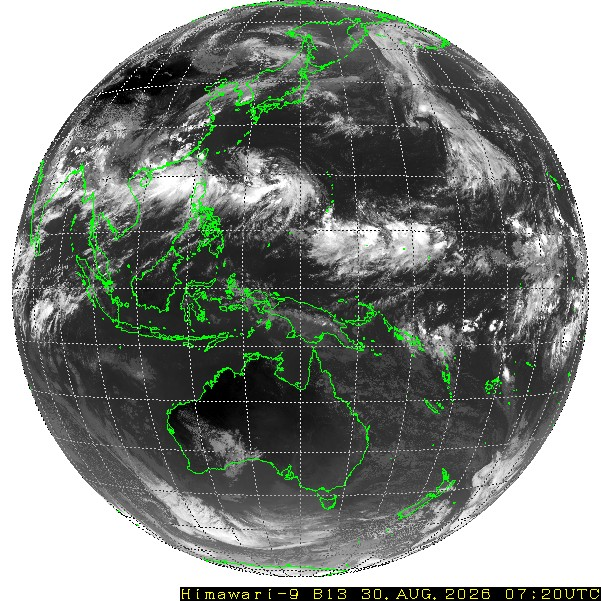
\includegraphics[width=0.61\textwidth]{figures/sky-witness.jpg}
\caption{The exact JMA Himawari full-disk Band 13 infrared JPEG published with the first production v1.2 seal. The signed metadata records the 07:10 UTC observation slot/scan start; the rendered JMA annotation shows 07:20 UTC, consistent with completion of a roughly ten-minute full-disk scan. Image SHA-256: \code{db39b531\ldots b6e3f6318}. Image attribution: Japan Meteorological Agency (JMA) \cite{jma2026,jmaimage2026}.}
\label{fig:witness}
\end{figure}

The package contained all nine required files. Independent execution of the reference publication verifier returned \code{"ok": true}, the expected ORCID identity, an entry count of one, and \code{sky_witness.artifacts_checked = true}. This verifies that the public JPEG digest equals the image digest inside the Passkey-approved canonical payload. At the immediate report-generation check, the two OpenTimestamps files were present but were treated as \code{pending_or_unverified}; no Bitcoin upper-bound claim should be made until a later \code{ots verify} succeeds. The production upgrade timer is designed to replace pending proofs after confirmation.

Operator logs recorded successful approval, local publication, owner-ledger synchronization, and GitHub mirroring. The public package is available at:

\begin{center}
\url{https://proof.excyberlab.net/proofs/01a05193-b0c5-7111-a71b-a6b1f982f748}.
\end{center}

\section{Discussion}

\subsection{Relevance in an era of generative systems}

When text, images, code, and analyses can be generated or altered at low cost, appearance alone becomes weak evidence of history. SkySeal does not attempt to classify a file as human- or AI-generated. Instead, it creates a durable statement about exact bytes, an approving credential, a persistent researcher identifier, and temporal evidence. This supports a different question: ``Were these exact bytes already included in this researcher's approved commitment by the verified upper-bound time?''

This distinction matters. Provenance evidence cannot replace assessment of originality or scientific validity, but it can make later fabrication, substitution, and date claims easier to evaluate. The posthumous audit model is particularly useful: public cryptographic material can outlive private accounts and can be checked without asking the original operator to sign a new statement.

\subsection{Why the sky witness matters}

The Himawari image is not merely a logo or decorative attachment. Its digest is inside the Passkey-signed payload, so the exact view of Earth is inseparable from the seal without invalidating the signature. It gives a human observer a recognizable physical context and makes the name ``SkySeal'' technically literal.

Its evidential role must nevertheless remain modest. A physical scene is not automatically a secure clock. The current implementation relies on JMA, HTTPS, response headers, and agent validation. Its strongest contribution is the combination of interpretability, global environmental context, and a conditional lower bound. OpenTimestamps remains necessary for an independently verifiable upper bound. The resulting two-sided model in Equation~\ref{eq:interval} is more informative than either component alone, provided the asymmetric trust assumptions are stated.

\subsection{Operational trade-offs}

Privacy minimization and user intelligibility pull in opposite directions. Omitting names and paths reduces disclosure, but a Passkey approval screen cannot display the file name that the user believes is being sealed. The private ledger restores this correspondence for the owner through a signed commitment, yet the public auditor cannot see it unless it is deliberately disclosed. Future interfaces could display a locally generated confirmation on a trusted owner device without sending the name to the public service.

The sorted-digest set also favors privacy and simplicity over structure. It makes a multi-file directory independently auditable when all bytes are disclosed, but it does not preserve internal organization or duplicate counts. A future version could support optional, salted hierarchical commitments while keeping v1's minimal public mode.

\section{Future work}

The following extensions would strengthen the system without changing the narrow v1.2 claim.

\begin{enumerate}
  \item \textbf{Stronger sky provenance.} Prefer a JMA product carrying a stable dated identifier or provider signature, retain verifiable HTTP metadata, explicitly represent scan start and completion, or combine independent Earth-observation sources. This would reduce dependence on a date-reused URL and a single provider.
  \item \textbf{Public transparency log.} Append seal manifests to an independently witnessed Merkle log so that deletion and equivocation across VPS and GitHub replicas are easier to detect.
  \item \textbf{Algorithm agility.} Define versioned commitments for future hash and signature algorithms, together with a migration procedure that preserves old evidence.
  \item \textbf{Credential lifecycle.} Complete append-only credential rotation, revocation, recovery, and multi-device policy while preserving the historical public key needed for old seals.
  \item \textbf{Reproducible verifier releases.} Publish signed source releases, locked dependencies, container or standalone builds, deterministic test vectors, and archival DOIs.
  \item \textbf{Long-term estate procedure.} Document how an executor can preserve candidate files, public evidence, optional receipts, and independent verifier instructions without access to the original Passkey.
  \item \textbf{Private mapping protection.} Replace the application-level private Sheet with client-side encrypted receipts or threshold disclosure for higher-confidentiality deployments.
  \item \textbf{Interoperability.} Explore exporting a SkySeal verification result as a C2PA assertion or other standard provenance envelope while retaining the private-source commitment model.
\end{enumerate}

\section{Conclusion}

SkySeal is an operational timestamping system for private research files. It binds exact byte commitments to an authenticated ORCID identity and an explicit User-Verified Passkey assertion, publishes self-contained evidence, and anchors that evidence through OpenTimestamps. Version 1.2 adds a signed digest of a recent JMA Himawari full-disk infrared image, making a state of the sky part of the approved digital record.

The system's value lies in the composition and separation of claims. The Passkey says which activated credential approved the payload; ORCID says which researcher identifier authenticated during enrollment; SHA-256 fixes exact bytes; the sky witness supplies conditional physical context and a lower temporal bound; OpenTimestamps supplies an independently verifiable upper bound after confirmation; and redundant public copies support later audit. None of these layers alone proves authorship or exact creation time. Together, with their limits stated, they provide a durable and practical research-provenance record suitable for independent and posthumous verification.

\appendix

\section{Independent verification procedure}

The following procedure verifies a disclosed candidate using a clone of the public repository. Python 3.10 or later, the \code{cryptography} package, and OpenTimestamps client 0.7.2 are required.

\begin{lstlisting}
git clone https://github.com/kagaya/SkySeal.git
cd SkySeal
python3 -m venv .venv-audit
. .venv-audit/bin/activate
python3 -m pip install -r verifier/requirements.txt \
  opentimestamps-client==0.7.2

python3 verifier/skyseal_find.py \
  /path/to/disclosed-file ./evidence

python3 verifier/skyseal_publication_verify.py \
  ./evidence/YYYY/MM/<seal-id> \
  --rp-id proof.excyberlab.net \
  --origin https://proof.excyberlab.net
\end{lstlisting}

A final report should require:

\begin{itemize}
  \item \code{"ok": true};
  \item the expected ORCID identity;
  \item successful User Present and User Verified checks in the bundle verifier;
  \item \code{sky_witness.artifacts_checked = true} for a v1.2 package;
  \item \code{confirmed} for both OpenTimestamps proofs before making the independent upper-bound claim.
\end{itemize}

Before Bitcoin confirmation, \code{--allow-pending-ots} verifies all other layers but must be reported as lacking an independently confirmed upper time bound.

\section{Private receipt verification}

If the owner discloses the exact \code{receipt_json} from the private ledger, save it as \code{receipt.json} and run:

\begin{lstlisting}
python3 verifier/skyseal_private_ledger_verify.py \
  receipt.json \
  ./evidence-directory/seal.skyseal.json \
  ./owner-disclosed-file-or-directory
\end{lstlisting}

This additional check validates the salted receipt commitment and the complete candidate hash set. It reveals the selected private Drive name and ID in the verifier report and should therefore be run only inside the agreed audit boundary.

\section{Claim checklist for auditors}

\begin{longtable}{>{\raggedright\arraybackslash}p{0.49\textwidth}>{\centering\arraybackslash}p{0.16\textwidth}>{\raggedright\arraybackslash}p{0.26\textwidth}}
\toprule
Statement & Supported? & Required evidence \\
\midrule
\endhead
Exact candidate bytes are in the approved set. & Yes & Candidate hash, strict hash list, signed bundle. \\
The approving credential is bound to the stated authenticated ORCID. & Yes & Genesis and activation verification. \\
The user was present and locally verified during approval. & Yes & WebAuthn UP and UV flags plus signature. \\
The exact published Himawari image was included in the approval. & Yes & Signed witness object, JPEG digest, manifest. \\
The signed evidence existed before a Bitcoin-attested time. & Yes, after confirmation & Successful verification of \nolinkurl{seal.skyseal.json.ots}. \\
The ORCID holder intellectually authored the work. & No & Requires external authorship evidence. \\
The file was first created at \code{created_at}. & No & \code{created_at} is informational. \\
The public seal identifies the original file name or Drive path. & No & Requires optional owner-disclosed receipt. \\
The candidate was the only file in a multi-hash seal. & No & Public set omits mapping and multiplicity. \\
The sky image alone is a trustless timestamp. & No & JMA/provider and capture trust remain. \\
\bottomrule
\end{longtable}

\bibliographystyle{plain}
\bibliography{skyseal-report}

\end{document}
